\section{Auswertung}


\begin{figure}
	\centering
	\begin{subfigure}{0.49\linewidth}
		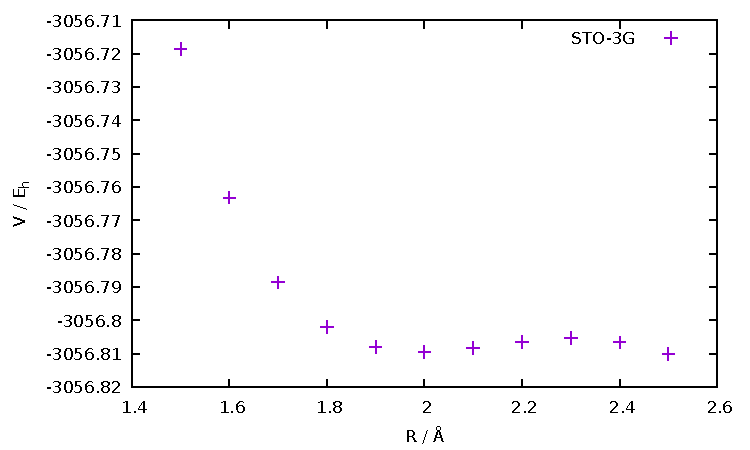
\includegraphics[width=\linewidth]{STO.pdf}
		\subcaption{Scanergebniss nach dem STO-3G Datensatz}
		\label{abb:STO}
	\end{subfigure}
	\hfill
	\begin{subfigure}{0.49\linewidth}
		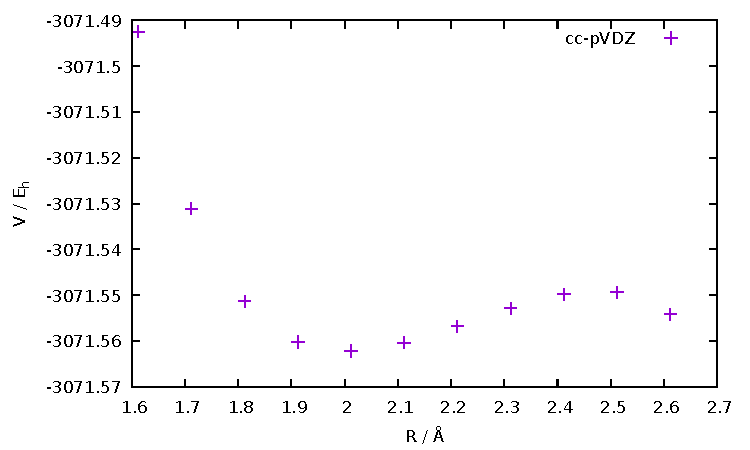
\includegraphics[width=\linewidth]{cc.pdf}
		\subcaption{Scanergebniss nach dem cc-pVDZ Datensatz}
 		\label{abb:cc}
	\end{subfigure}
	\caption{Totale Energie über Abstand der Reaktionspartner entlang der Reaktionskoordinate}
\end{figure}
Nach beendigung der Simulationen sind die in den Abbildungen \ref{abb:STO} und \ref{abb:cc}, sowie der Tabelle \ref{tab:AusgDaten} enthaltenen Daten erhalten worden.
Wie hier Zusehen wurden als erstes Nicht-SI-Einheiten in SI-Einheiten umgerechnet. 
Außerdem ist die elektronische Energie mit der Avogadrozahl multipliziert worden, um später eine molare Reaktionsenthalpie zu erhalten.
Dies vereinfacht im Weitern die Vergleichbarkeit.
Nach Gleichung \ref{eq:rktEnth} ist die Summe aus elektrischer Energie und die Nullpunktsschwingungsenergie die Reaktionsenthalpie.
\begin{equation}
H=EE+ZPVE
\label{eq:rktEnth}
\end{equation}

\begin{table}{b}
\centering
\begin{tabular}{rl|cccc}
Basissatz&         				& STO-3G              & STO-3G              & Cc-pVDZ             & Cc-pVDZ\\
Zustand	 &           				& Produkt             & Übergangszustand    & Produkt             & Übergangszustand\\
\hline
\hline
EE       &/\unit{\hartree} 			& -3038,27            & -3038,26            & -3071,58            & -3071,55\\
EE       &/\unit{\mega\joule\per\mole}   	& -7976,898           & -7976,866           & -8064,336           & -8064,268\\
ZPVE     &/\unit{\hartree}    			& 0,044               & 0,044               & 0,040               & 0,039\\
ZPVE     &/\unit{\joule\per\mole} 		& 116560,49	      & 115011,46           & 105685,78           & 102511,58\\
T        &/\unit{\kelvin}                	& 298,15              & 298,15              & 298,15              & 298,15\\
S        &/\unit{\cal\per\mole\per\kelvin}    	& 78,242              & 70,352              & 28,647              & 73,321\\
S        &/\unit{\joule\per\mole\per\kelvin}	& 327,36              & 294,35              & 119,86              & 306,78\\
\end{tabular}
\caption{Ausgangsdaten nach der Simulation der Reaktion}
\label{tab:AusgDaten}
\end{table}  

Weiter kann über die Gibbs-Gleichung (Gleichung \ref{eq:gibbs}) die gleichnamige Enthalpie (oder auch freie Reaktionsenthalpie genannt) errechnet werden.
\begin{equation}
G=H-T\Delta S
\label{eq:gibbs}
\end{equation}
Die Differenz der Gibbs-Energien zwischen Produkt und Übergangszustand gibt die Aktivierungsenergie.
Diese kann nun über die Arrheniusgleichung (Gleichung \ref{eq:arr}) in die dazugehörige Geschwindigkeitskonstante umgerechnet werden.
\begin{equation}
k=e^{\frac{-E_A}{R\cdot T}}
\label{eq:arr}
\end{equation}
Die Resultate dieser Rechnungen sind in Tabelle \ref{tab:res} dargestellt.
Der cc-pVDZ Basissatz ist generell größer und damit genauer.
Der STO-3G Datensatz zielt darauf ab, mit mathematischen Vereinfachungen einen Effizienten Überblick über die Energien zu bekommen \cite{sto}.
Während der cc-pVDZ Datensatz entwickelt wurde, mit dem Anspruch, möglichst komplett zu sein \cite{cc}.
Dies spiegelt sich zum Beispiel auch in der Rechenzeit wieder, welche hier deutlich länger gedauert haben. 
Zusehen ist dieser Unterschied unter anderem an den geringeren Energien, welche der cc-pVDZ Datensatz errechnet hat.
Nach dem Variationstheorem wird davon ausgegangen, das solche Simulationen stets einen zu großen Energiewert errechnen.
Somit sind niedrigere Ergebnisse immer näher an dem wahren Wert.
Weiter ist die errechnete Aktivierungsenergie sehr nah an den Literaturwerten.
Nach Tabelle \ref{tab:res} wurde über den cc-pVDZ Datensatz eine Aktivierungsenergie von \qty{9359,084}{\joule\per\mole} ermittelt werden.
Nach diesem\cite{geschk} Paper wird für diese Reaktion eine Aktivierungsenergie von \qty{-1,9}{\kilo\cal\per\mol} oder \qty{-7949,6}{\joule\per\mole}

\begin{table}
\centering
\begin{tabular}{rl|cccc}
\multicolumn{2}{c}{Basissatz}		   	& STO-3G        & STO-3G              & Cc-pVDZ              & Cc-pVDZ\\
\multicolumn{2}{c}{Zustand}			& Produkt       & Übergangszustand    & Produkt              & Übergangszustand\\
\hline
\hline
$H$             &/\unit{\mega\joule\per\mole} 	& -7976,78        & -7976,751   & -8064,231    & -8064,166\\
$G$             &/\unit{\mega\joule\per\mole}   & -7976,88        & -7976,839   & -8064,266    & -8064,257\\
$E_A$           &/\unit{\joule\per\mole} 	& \multicolumn{2}{c}{-40324,19}	& \multicolumn{2}{c}{-9359,084}\\
$k$             &/\unit{\per\second}       	& \multicolumn{2}{c}{\qty{8,62e-08}{}} & \multicolumn{2}{c}{0,0229}\\
\end{tabular}
\caption{Ergebnisse}
\label{tab:res}
\end{table}

